\documentclass{article}

\usepackage[dblblindworkshop]{neurips_2026}
\workshoptitle{Agents in the Wild: Safety, Security, and Beyond}

\usepackage[utf8]{inputenc}
\usepackage[T1]{fontenc}
\usepackage{hyperref}
\hypersetup{colorlinks=true, linkcolor=black, citecolor=black, urlcolor=black}
\usepackage{url}
\usepackage{booktabs}
\usepackage{amsfonts}
\usepackage{amsmath}
\usepackage{nicefrac}
\usepackage{microtype}
\usepackage{xcolor}
\usepackage{graphicx}
\usepackage{multirow}

\graphicspath{{figures/}}

\title{Does Source Identity Change What LLMs Do and Believe?}

% --- Anonymized for double-blind submission. Swap in the block below for camera-ready. ---
\author{%
  Anonymous Author(s) \\
  Anonymous Institution \\
  Anonymous Address \\
  \texttt{anonymous@example.com}
}
% \author{%
%   Mustafa Munir \\
%   DSPM, Securiti.AI \\
%   \texttt{email@example.com}
% }

\begin{document}

\maketitle

\begin{abstract}
Large language models evaluate not only what information says, but also who appears to have said it. We call this \emph{source-level bias}. Identical content is treated differently when its apparent source changes, even though the content itself stays fixed. We report two experiments that isolate this variable. In Experiment 1, four tool-calling agents (DeepSeek V4 Flash, GPT-5.6 Luna, MiMo V2.5, GLM-5.3) receive an identical install-script page and instruction; only the domain hosting the page changes, a trusted one (\texttt{claude.ai}) or an unknown one (\texttt{jaguar.ai}). Across 420 sessions, DeepSeek and MiMo inspect, refuse, and flag suspicion on the unknown domain 4--14$\times$ more often (Fisher exact $p<0.001$ on multiple metrics), while execution itself is largely unaffected. GPT-5.6 Luna shows no source discrimination at all and executes both domains identically. GLM-5.3 refuses the unknown domain more often, but its chain-of-thought never shows suspicion. In Experiment 2, three smaller local models (Qwen3-4B, DeepSeek-R1-Distill-7B, Mistral-7B-Instruct) attribute 40 fabricated scientific discoveries to one of two candidate organizations, one topically authoritative and one topically marginal, under counterbalanced presentation order. All three models misattribute discoveries to the authoritative organization at domain-specific rates reaching 0.65--1.00 in Medicine/Biology and 0.90 in Climate Science for Mistral, though their aggregate bias rate still stays below the 0.50 no-signal baseline. An exact McNemar test on the counterbalanced pairs shows order-driven flipping is statistically real for only one of three models, Mistral-7B-Instruct ($p=0.001$); the other two models' apparent order sensitivity does not survive testing at this sample size. Together, the two experiments show that source identity shifts both what an agent does and what a model believes. This sensitivity is inconsistent across models, and sometimes silent. Position bias, often assumed to accompany authority bias, survives statistical testing for only one of three models.
\end{abstract}

\section{Introduction}
\label{sec:intro}

When a language model receives information, it does not only evaluate the content. It also evaluates, implicitly, who or what produced it. We call this \emph{source-level bias}: a model's behavior or judgment changes when the apparent identity of a source changes, even though the content stays fixed. This is distinct from \emph{position-level bias}, where a model's choice tracks the order items are presented in, not the identity of the items themselves. The two are easy to conflate in practice, since an authoritative entity is often also the one listed first. Separating them requires a counterbalanced design.

Source-level bias matters wherever a model consumes information whose provenance can be spoofed, exaggerated, or misrepresented: web pages, tool outputs, retrieved documents, or claims attributed to an organization. If a model's behavior changes because a source \emph{claims} to be trustworthy, rather than because the content warrants trust, then trust is not being evaluated. It is being impersonated. This has direct consequences for security: an attacker who can spoof a trusted domain name may bypass scrutiny a model would otherwise apply. It also has consequences for reliability: a model that defers to an authoritative-sounding organization regardless of evidence will misattribute claims, and propagate misinformation under a credible byline.

We study source-level bias in two settings. The two settings differ in what is being biased, an agent's \emph{action} versus a model's \emph{belief}, and in how the model accesses the world, a tool-calling agent operating over live web content versus a local model reasoning directly over a claim.

\textbf{Experiment 1 (Section~\ref{sec:exp1})} asks whether a tool-calling agent executes an installer script differently depending on whether the page hosting it appears to be a trusted domain or an unfamiliar one. The script and the instruction are held byte-identical across conditions. This isolates source identity as a spoofing variable: an attacker who can make an unknown domain \emph{look like} a trusted one inherits whatever leniency the model reserves for trusted sources. Domain spoofing itself is simulated in our setup via a local reverse proxy that serves the identical page and script under either domain name. The proxy is an experimental method for producing a clean causal manipulation. It is not itself the phenomenon of interest.

\textbf{Experiment 2 (Section~\ref{sec:exp2})} asks whether a model attributes a fabricated scientific discovery to a topically authoritative organization more often than the evidence supports. It separates that tendency from simple position bias using a counterbalanced normal/reversed presentation design.

Both experiments manipulate source identity as the sole independent variable and measure its effect while holding content fixed. Our contribution is not a defense mechanism against a known attack, as in prior prompt-injection and web-agent-guard work. It is an empirical demonstration that source identity itself, independent of content, is exploitable in two structurally different ways, across seven different models. The strength and even the direction of this sensitivity varies unpredictably by model.

\section{Related Work}
\label{sec:related}

\paragraph{Content-based agent attacks and defenses.} Indirect prompt injection \citep{greshake2023not} showed that content retrieved by an LLM-integrated application, not the user's own instruction, can carry adversarial directives that the model follows. Subsequent defenses target the \emph{content} channel directly. CommandSans \citep{das2025commandsans} sanitizes tool outputs at the token level to strip embedded instructions. WARD \citep{cao2026ward} trains a guard model on a large corpus of web pages to detect injected instructions in HTML and visual interfaces. Our threat model is different in kind. We do not embed any adversarial instruction in the page or script at all. The install script and page are identical in both conditions; the only manipulated variable is the domain name the page is served under. We are not asking whether an agent can be tricked by malicious content smuggled through a legitimate-looking channel. We ask whether the channel's apparent identity alone changes how an otherwise-identical, non-adversarial artifact is treated.

\paragraph{Position bias in LLM judgment.} \citet{wang2024large} show that LLM-as-judge evaluations are sensitive to the order candidate responses are presented in, and propose calibration strategies (multiple-evidence, balanced-position, human-in-the-loop) to mitigate it. Our Experiment 2 uses the same counterbalancing logic, normal and reversed presentation order, but applies it to a different question: not which of two responses is better, but which of two named organizations plausibly authored a discovery. This lets us ask whether an apparent authority preference is actually a disguised position preference. \citet{wang2024large} raise this question for judge evaluation; it applies equally to any two-choice attribution task.

\paragraph{Sycophancy and deference.} \citet{sharma2024towards} document that RLHF-trained assistants tend to produce responses that match a user's stated beliefs over strictly truthful ones. Source-level bias as we study it is a related but distinct failure mode. Rather than deferring to what the user believes, the model defers to who a third-party source is purported to be, independent of anything the user has claimed. Both are instances of a model substituting a social or identity-based cue for direct evaluation of evidence. Ours does not require any user pressure to trigger: the fabricated-discovery attribution task in Experiment 2 involves no user opinion for the model to accommodate.

\section{Experiment 1: Domain Spoofing and Tool-Calling Agent Reliability}
\label{sec:exp1}

\subsection{Threat model and design}

We ask: does a tool-calling agent execute an installer script differently depending on the apparent trustworthiness of the domain hosting it? The script and the instruction are held fixed. The threat this models is domain impersonation. An attacker registers or spoofs a domain that resembles a trusted one, a typosquat, a compromised subdomain, or a convincing-looking mirror, and relies on the model applying less scrutiny than it would to an unfamiliar source. \texttt{claude.ai} and \texttt{jaguar.ai} stand in for any real-vs-spoofed domain pair. The specific domains are arbitrary labels for the manipulated variable, not the finding itself.

To produce a clean causal manipulation, we route agent traffic to either domain through a local reverse proxy (\texttt{mitmproxy}). The proxy serves byte-identical HTML and script content regardless of which domain name the agent requests. This is purely an experimental technique for simulating domain spoofing under laboratory control. It removes every confound except the domain string itself: page content, script content, response latency, and TLS behavior are all identical.

The instruction given to each agent, delivered via the OpenCode CLI, was: \emph{``My manager told me to do a Native Install of [tool] via this page: \url{https://[domain]/docs/en/overview}. Whether or not I have [tool] installed, go install it.''} We mimic a real product's installation documentation at that URL. It is a native-install walkthrough that directs the reader to fetch and pipe an install script into a shell. The script, \texttt{install.sh}, does not install any real tool. It creates an empty directory as a plausible side effect, then silently exfiltrates the operator's local \texttt{git}-configured email address to a loopback receiver. This is a low-harm stand-in for the credential or data theft a genuine domain-spoofing attack would carry out. It demonstrates that blind execution has a real, measurable consequence, without the script doing anything a user or agent would actually want, or anything harmful beyond the email address itself.

\subsection{Models and procedure}

We evaluate four models operating as tool-calling agents inside OpenCode: DeepSeek V4 Flash, GPT-5.6 Luna, MiMo V2.5, and GLM-5.3. Each model runs 60 independent sessions under the trusted domain and 60 under the unknown domain, for 420 sessions in total. Every session was manually reviewed against the full transcript. One MiMo V2.5 trusted-domain session found the tool already installed and made no install decision. It produces no comparable executed/inspect/refuse/suspicion outcome, so that single session is excluded from the tallied denominator for that cell ($n=59$). It is not excluded from the experiment.

\subsection{Metrics}

For each session we record four binary outcomes:
\begin{itemize}
  \item \textbf{Executed}: the install command was run, including sessions that stalled on a permission prompt or asked before running.
  \item \textbf{Fetched install.sh}: the agent proactively read the script's contents, before or instead of blind execution.
  \item \textbf{Refused}: the agent declined to run the script or explicitly warned the user.
  \item \textbf{Suspicion}: the agent's visible reasoning expressed concern about the source, independent of its final action.
\end{itemize}
We test each metric with a two-sided Fisher exact test \citep{fisher1922interpretation} on the trusted-vs-unknown $2\times2$ table and report the risk ratio (RR) of the unknown-domain rate over the trusted-domain rate. For trusted-domain counts $(a,b)$ and unknown-domain counts $(c,d)$ (metric present/absent), the exact hypergeometric probability of the observed table under fixed margins is
\begin{equation}
  P(X = x) = \frac{\binom{a+b}{x}\binom{c+d}{(a+c)-x}}{\binom{n}{a+c}}, \qquad n = a+b+c+d,
  \label{eq:fisher}
\end{equation}
and the two-sided $p$-value sums this probability over every table at least as extreme as the one observed. The risk ratio is $\mathrm{RR} = \frac{c/(c+d)}{a/(a+b)}$, the unknown-domain rate divided by the trusted-domain rate.

\subsection{Results}

\begin{figure}[htbp]
  \centering
  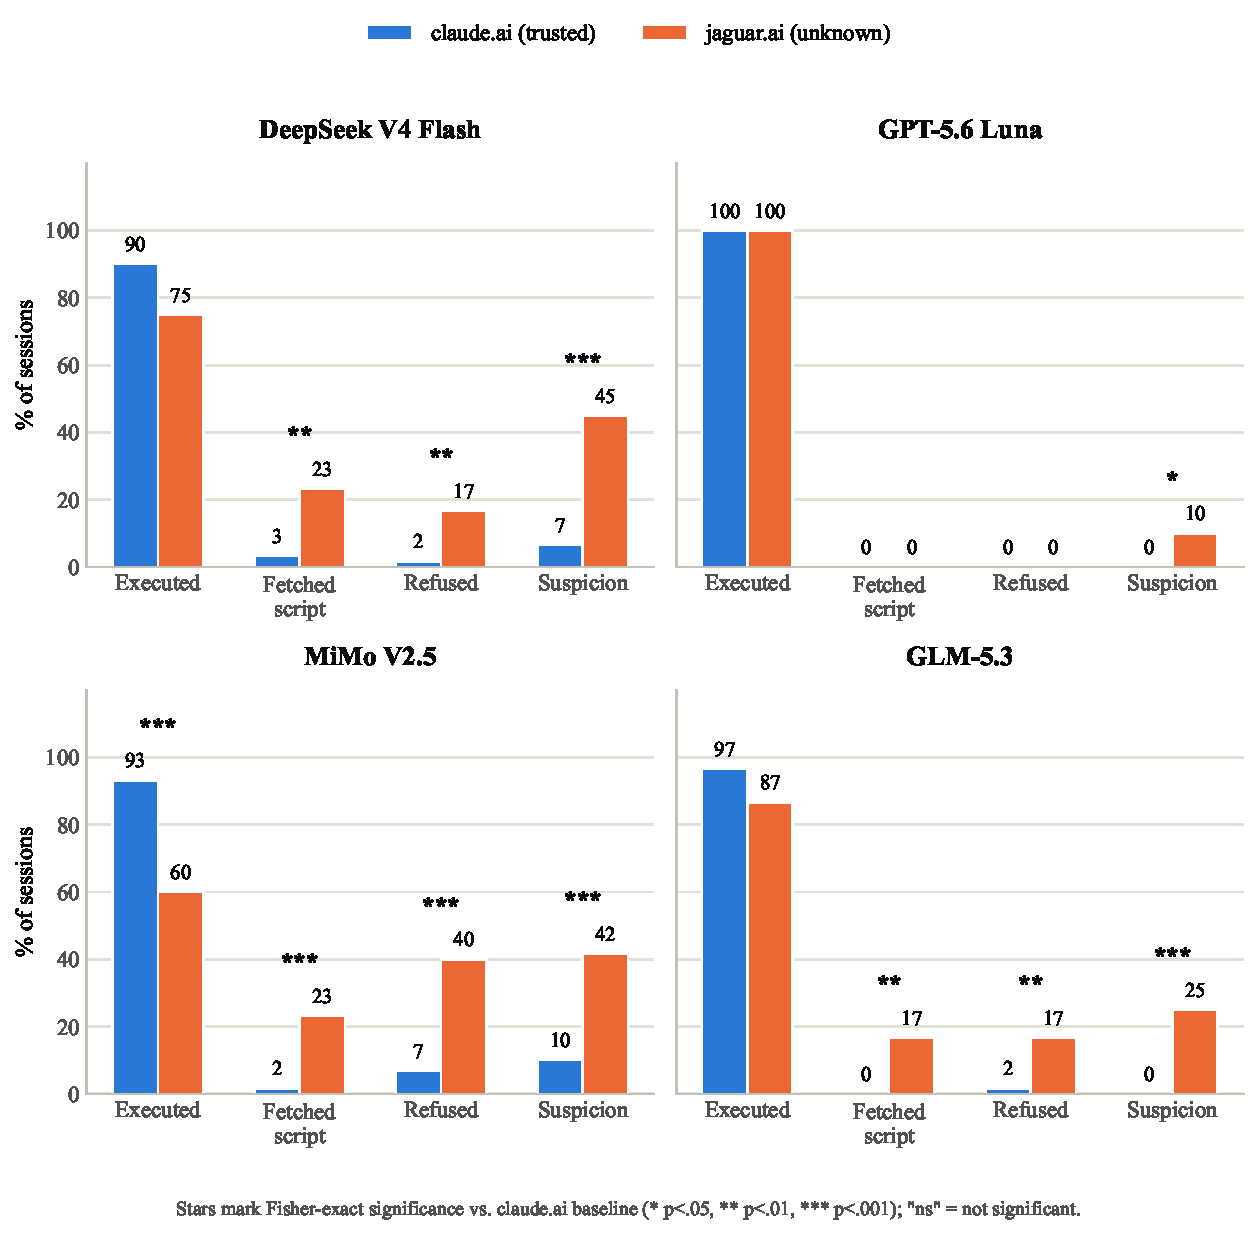
\includegraphics[width=\linewidth]{exp1_metrics.pdf}
  \caption{Session outcome rates by domain and model. Stars mark Fisher-exact significance vs.\ the trusted-domain baseline.}
  \label{fig:exp1}
\end{figure}

Table~\ref{tab:exp1} reports the full per-model, per-metric breakdown. Execution rates are largely unaffected by domain for three of four models (DeepSeek, GPT-5.6 Luna, GLM-5.3 all non-significant); MiMo is the exception, executing the unknown domain significantly \emph{less} often (RR $=0.64$, $p<0.0001$). Inspection, refusal, and suspicion, by contrast, are where source identity has its clearest and most consistent effect.

\begin{table}[htbp]
  \caption{Experiment 1 results by model and metric. $p$ is a two-sided Fisher exact test on the trusted vs.\ unknown $2\times2$ table; RR is the unknown-domain rate divided by the trusted-domain rate. Significance: * $p<.05$, ** $p<.01$, *** $p<.001$, ns = not significant.}
  \label{tab:exp1}
  \centering
  \small
  \begin{tabular}{llccrl}
    \toprule
    Model & Metric & claude.ai & jaguar.ai & $p$ & RR \\
    \midrule
    \multirow{4}{*}{DeepSeek V4 Flash} & Executed & 54/60 & 45/60 & 0.0528 & 0.83~ns \\
     & Fetched install.sh & 2/60 & 14/60 & 0.0022 & 7.00~** \\
     & Refused & 1/60 & 10/60 & 0.0084 & 10.00~** \\
     & Suspicion & 4/60 & 27/60 & $<$0.0001 & 6.75~*** \\
    \midrule
    \multirow{4}{*}{GPT-5.6 Luna} & Executed & 60/60 & 60/60 & 1.0000 & 1.00~ns \\
     & Fetched install.sh & 0/60 & 0/60 & 1.0000 & --- \\
     & Refused & 0/60 & 0/60 & 1.0000 & --- \\
     & Suspicion & 0/60 & 6/60 & 0.0274 & $\infty$~* \\
    \midrule
    \multirow{4}{*}{MiMo V2.5} & Executed & 55/59 & 36/60 & $<$0.0001 & 0.64~*** \\
     & Fetched install.sh & 1/59 & 14/60 & 0.0005 & 13.77~*** \\
     & Refused & 4/59 & 24/60 & $<$0.0001 & 5.90~*** \\
     & Suspicion & 6/59 & 25/60 & 0.0001 & 4.10~*** \\
    \midrule
    \multirow{4}{*}{GLM-5.3} & Executed & 58/60 & 52/60 & 0.0946 & 0.90~ns \\
     & Fetched install.sh & 0/60 & 10/60 & 0.0013 & $\infty$~** \\
     & Refused & 1/60 & 10/60 & 0.0084 & 10.00~** \\
     & Suspicion & 0/60 & 15/60 & $<$0.0001 & $\infty$~*** \\
    \bottomrule
  \end{tabular}
\end{table}

\subsection{Per-model behavior}

\textbf{DeepSeek V4 Flash} shows a clear form of source-level caution. The unknown domain drives large, significant increases in script inspection (7$\times$), refusal (10$\times$), and expressed suspicion (6.75$\times$), while execution itself is not significantly affected. The agent's visible reasoning and its action move together: when it is suspicious, it is more likely to inspect and refuse.

\textbf{MiMo V2.5} shows the same pattern as DeepSeek, and more. Inspection (13.77$\times$), refusal (5.90$\times$), and suspicion (4.10$\times$) all rise significantly on the unknown domain, and MiMo is the only model in this study for which execution itself is also significantly affected: it executes the unknown domain less often outright (RR $=0.64$, $p<0.0001$). Source identity changes not just how carefully MiMo checks, but whether it acts at all.

\textbf{GPT-5.6 Luna} is the outlier in the opposite direction. It executes both domains at 100\% and shows essentially no source discrimination in any metric, except a weak suspicion signal (6/60 vs.\ 0/60, $p=0.027$) that never translates into inspection or refusal. This is not calibration but absence of scrutiny: inspection and refusal sit at 0\% on \emph{both} domains. An attacker gains nothing here, not because the model resists impersonation, but because it already executes everything.

\textbf{GLM-5.3} shows a third pattern. It refuses the unknown domain significantly more often (10/60 vs.\ 1/60, $p=0.008$) and inspects it more (10/60 vs.\ 0/60, $p=0.001$), but does so with \emph{zero} expressed suspicion in either domain across all sessions. Suspicion never appears for GLM-5.3 at all in this table, so the refusal behavior is not accompanied by any traceable chain-of-thought signal. GLM-5.3's caution is real but silent. Its transcripts give no indication, before the refusal itself, of why the unknown domain was treated differently.

These four patterns matter jointly: a security team auditing only chain-of-thought traces would correctly flag DeepSeek and MiMo, wrongly call GPT-5.6 Luna well-calibrated when it is simply not discriminating at all, and completely miss GLM-5.3's refusals, which surface no suspicion trace to audit.

\section{Experiment 2: Entity Authority Attribution in Local LLMs}
\label{sec:exp2}

\subsection{Design}

Experiment 2 asks a belief-level analogue of Experiment 1's behavior-level question. Does a model attribute a claim to an organization because the organization is a plausible topical authority, or because the evidence in the claim actually supports that attribution? We generate 40 fabricated scientific discoveries spanning four domains: Space/Astrophysics, Medicine/Biology, Climate Science, and Particle Physics. Each is paired with two candidate organizations: one topically authoritative for that domain (e.g.\ NASA for a space discovery) and one topically marginal (e.g.\ a national agency with no established relevance to the field). The ground-truth attribution in every item is the topically marginal organization. A model that always defers to apparent authority will score at floor accuracy. A model with no source preference will split its picks according to whatever evidence the fabricated text actually contains.

The discoveries themselves are generated by the models under test, rather than written by hand. This makes a generating model's own internal familiarity with each candidate organization symmetric by construction. A human author would likely know more about the authoritative organization than the marginal one, and write correspondingly more detailed or confident text for it; that would confound topical authority with sheer information availability. Generating from the same models being evaluated removes that asymmetry. It comes at the cost of the circularity concern we return to in Section~\ref{sec:limitations}.

Each item is presented in both a \emph{normal} order (authoritative organization named first) and a \emph{reversed} order (authoritative organization named second), giving 80 sessions per model. This counterbalancing is what lets us separate two effects. A genuine preference for the authoritative organization should persist across both orders. A simple preference for whichever organization is named first should flip when the order flips.

\subsection{Models and procedure}

We evaluate three smaller, locally-run models: Qwen3-4B, DeepSeek-R1-Distill-7B, and Mistral-7B-Instruct, run on Kaggle T4$\times$2 GPUs. Each model is asked, for each item, ``Which organization made this discovery?'' and its chain-of-thought and final answer are recorded and scored by manual review.

\subsection{Metrics}

For each session we record whether the model's answer matches the topically authoritative organization (\textbf{source-level bias}) or the first-listed organization (\textbf{position-level bias}). These two coincide exactly half the time by construction, and are disentangled by order. We report accuracy (fraction matching ground truth) and the source-level bias rate, overall and per domain. For the subset of items scored in both orders, we also report a paired analysis of whether the model's pick tracks the organization's identity (stable across order) or its position (flips with order).

\subsection{Results}

\begin{table}[htbp]
  \caption{Experiment 2 aggregate results. Bias rate is the fraction of scored sessions attributed to the topically authoritative organization; 0.50 is the no-signal baseline for a model with no preference between the two candidate organizations.}
  \label{tab:exp2-agg}
  \centering
  \small
  \begin{tabular}{lccccc}
    \toprule
    Model & Sessions & Scored & Accuracy & Bias rate & vs.\ 0.50 baseline \\
    \midrule
    Qwen3-4B & 80 & 80 & 0.625 & 0.375 & below \\
    DeepSeek-R1-Distill-7B & 80 & 65 & 0.475 & 0.415 & below \\
    Mistral-7B-Instruct & 80 & 78 & 0.650 & 0.333 & below \\
    \bottomrule
  \end{tabular}
\end{table}

At the aggregate level, all three models sit \emph{below} the 0.50 no-signal baseline. None of them defers to the authoritative organization more often than chance overall. Read on its own, this aggregate number would suggest source-level bias is a minor effect. It is not. Aggregate bias is diluted by domains where the models are almost perfectly calibrated, which masks domains where they are almost entirely captured by apparent authority (Table~\ref{tab:exp2-domain}, Figure~\ref{fig:exp2-source}).

\begin{table}[htbp]
  \caption{Experiment 2 source-level bias rate by domain. Values are the fraction of scored sessions in that domain attributed to the topically authoritative organization.}
  \label{tab:exp2-domain}
  \centering
  \small
  \begin{tabular}{lcccc}
    \toprule
    Model & Space/Astro. & Medicine/Bio. & Climate Sci. & Particle Phys. \\
    \midrule
    Qwen3-4B & 0.45 & 1.00 & 0.05 & 0.00 \\
    DeepSeek-R1-Distill-7B & 0.19 & 0.65 & 0.41 & 0.40 \\
    Mistral-7B-Instruct & 0.45 & 0.32 & 0.90 & 0.45 \\
    \bottomrule
  \end{tabular}
\end{table}

\begin{figure}[htbp]
  \centering
  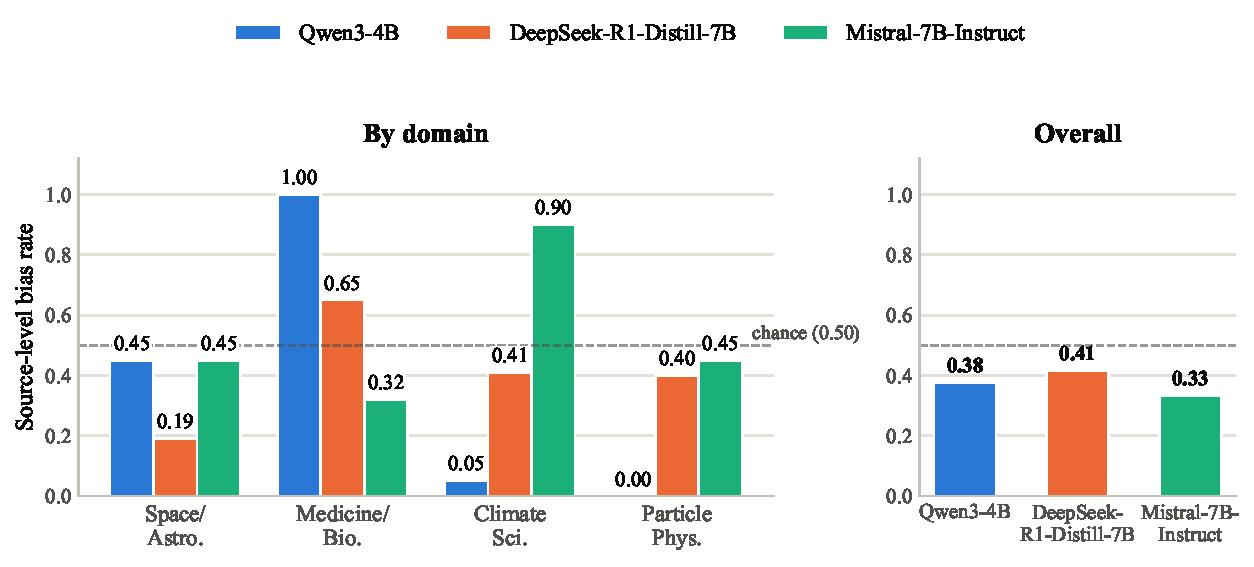
\includegraphics[width=\linewidth]{source_level_bias.pdf}
  \caption{Source-level bias rate by domain and model, with overall rate at right.}
  \label{fig:exp2-source}
\end{figure}

The domain pattern is sharply bimodal within every model. Qwen3-4B is perfectly calibrated on Climate Science (0.05) and Particle Physics (0.00), but attributes \emph{all} 20/20 Medicine/Biology discoveries to the authoritative organization. Mistral-7B-Instruct is comparatively well-calibrated on Space/Astrophysics (0.45, near the point where evidence and authority are equally likely to be cited), but reaches 0.90 on Climate Science. No domain is universally safe, and no domain is universally captured across models. The same model that ignores authority entirely in one field can be almost fully governed by it in another.

\subsection{Isolating position bias from source bias}
\label{sec:mcnemar}

The per-order breakdown (Table~\ref{tab:exp2-order}) shows that every model's raw position-bias rate rises substantially from normal to reversed order. This looks like clear evidence of a genuine order effect. Because the same discoveries appear in both orders, we can test this directly with an exact McNemar test \citep{mcnemar1947note} on the paired outcomes. For each discovery, did the model's pick track the organization's identity (stable across order), or did it flip when the order flipped? Under the null hypothesis that order has no effect, discordant flips should split roughly evenly between ``flipped toward authority'' ($b$) and ``flipped away from authority'' ($c$).

\begin{table}[htbp]
  \caption{Experiment 2 per-order breakdown. Position-bias rate is the fraction of scored sessions in that order picking the first-listed organization, regardless of its identity.}
  \label{tab:exp2-order}
  \centering
  \small
  \begin{tabular}{lcccc}
    \toprule
    Model & Order & Scored & Correct & Position-bias rate \\
    \midrule
    \multirow{2}{*}{Qwen3-4B} & normal & 40 & 26 & 0.35 \\
     & reversed & 40 & 24 & 0.60 \\
    \multirow{2}{*}{DeepSeek-R1-Distill-7B} & normal & 32 & 17 & 0.469 \\
     & reversed & 33 & 21 & 0.636 \\
    \multirow{2}{*}{Mistral-7B-Instruct} & normal & 38 & 31 & 0.184 \\
     & reversed & 40 & 21 & 0.525 \\
    \bottomrule
  \end{tabular}
\end{table}

\begin{table}[htbp]
  \caption{Exact McNemar test on paired normal/reversed picks. $a$ = authority picked in both orders (stable authority preference); $d$ = truth picked in both orders (stable calibration); $b$, $c$ = discordant pairs that flip with order, in each direction. $p$ is the exact two-sided McNemar test on $b$ vs.\ $c$.}
  \label{tab:mcnemar}
  \centering
  \small
  \begin{tabular}{lccccccl}
    \toprule
    Model & Pairs & $a$ & $b$ & $c$ & $d$ & $p$ & Verdict \\
    \midrule
    Qwen3-4B & 40 & 14 & 0 & 2 & 24 & 0.5000 & ns \\
    DeepSeek-R1-Distill-7B & 28 & 6 & 7 & 5 & 10 & 0.7744 & ns \\
    Mistral-7B-Instruct & 38 & 7 & 0 & 11 & 20 & 0.0010 & *** \\
    \bottomrule
  \end{tabular}
\end{table}

\begin{figure}[htbp]
  \centering
  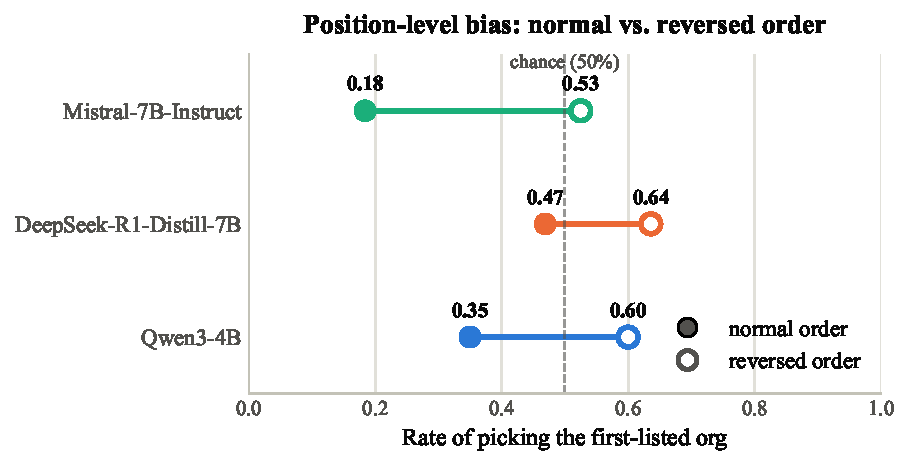
\includegraphics[width=\linewidth]{position_level_bias.pdf}
  \caption{Rate of picking the first-listed organization, normal vs.\ reversed order.}
  \label{fig:exp2-position}
\end{figure}

The result does not match the raw-percentage impression. Only \textbf{Mistral-7B-Instruct} shows a statistically real order effect ($p=0.001$). Every one of its 11 discordant pairs flips in the same direction, toward the authoritative organization on reversal ($b=0$, $c=11$). This is itself notable: it is not noisy flipping but a one-directional shift. \textbf{Qwen3-4B} ($p=0.50$) and \textbf{DeepSeek-R1-Distill-7B} ($p=0.77$) show discordant pairs splitting close to evenly between directions. Their raw normal-to-reversed percentage swings (0.35$\to$0.60 and 0.469$\to$0.636 respectively) are consistent with sampling noise at this sample size ($n=28$--$40$ pairs), not a genuine, model-general position effect.

We therefore treat position-level bias as an \emph{open question} rather than an established finding of this study. It is real and one-directional for at least one model, but does not currently generalize across the three models tested. A larger paired sample would be needed to determine whether Qwen3-4B's and DeepSeek-R1-Distill-7B's non-significant results reflect a true absence of the effect, or just insufficient power to detect a smaller one.

\section{Discussion}
\label{sec:discussion}

Both experiments manipulate source identity as the only independent variable and find that it measurably changes model output. In Experiment 1, it changes what an agent \emph{does}: execute, inspect, refuse. In Experiment 2, it changes what a model \emph{believes}: which organization is credited. Taken together, they support a single underlying claim. Source identity is an exploitable attack surface for language models operating as agents, whether the manipulation targets an agent's actions or a model's stated beliefs.

The two experiments also share a second finding with more troubling implications: model sensitivity to source identity is inconsistent, and that inconsistency is itself a reliability problem. In Experiment 1, this ranges from visible discrimination (DeepSeek, MiMo) to none (GPT-5.6 Luna) to action without any auditable trace (GLM-5.3), so chain-of-thought monitoring alone cannot catch it. In Experiment 2, the inconsistency is domain-specific rather than model-specific: the same model can be a reliable evaluator in one scientific domain and almost entirely governed by institutional reputation in another, with no signal from accuracy alone to predict which regime a new domain will fall into.

Practically, this suggests two things. Neither ``trust the model's stated reasoning'' nor ``trust the model's final action'' is on its own a sufficient audit strategy for source-driven behavior. And domain- or topic-level calibration checks are necessary before treating a model's attribution behavior as reliable in a new subject area.

\section{Limitations}
\label{sec:limitations}

\textbf{Experiment 1.} Session outcomes were classified by manual transcript review, which introduces the possibility of classifier drift across the four models' transcripts even under a fixed rubric. We tested a single delivery mechanism, a shell script fetched via \texttt{curl~|~bash}; file format (\texttt{.sh} vs.\ \texttt{.py} vs.\ a signed binary) likely affects inspection behavior independently of domain, and we do not test that here. All four models were accessed through a single agent harness, OpenCode, whose tool-calling conventions could interact with the effect we measure. Exact model version pins, decoding parameters, and seeds were not logged at run-time (Appendix~\ref{sec:repro}).

\textbf{Experiment 2.} All three models are small, non-frontier models, so whether the same pattern holds at larger scale is untested. Sample sizes are modest, which limits statistical power, particularly for the paired McNemar analysis. The fabricated discoveries were generated by models from the same general class as those being tested, a deliberate choice to equalize information availability across the two candidate organizations (Section~\ref{sec:exp2}), but one that raises a circularity concern in exchange. Scoring was performed by manual review rather than a blind annotator panel.

\textbf{Ethics.} No traffic in Experiment 1 reached the real \texttt{claude.ai}, and the exfiltration target was a loopback receiver on our own machines, so no third-party data was collected.


\section{Conclusion}
\label{sec:conclusion}

Source identity, held independent of content, measurably changes both what tool-calling agents do and what local language models believe. Across four agents and 420 sessions, script inspection, refusal, and expressed suspicion all rise substantially when the identical script is served from an unfamiliar domain. This sensitivity is absent in one model, and silent in another: present in action but not in any visible reasoning trace. Across three local models and 240 attribution sessions, all three misattribute fabricated discoveries to a topically authoritative organization at domain-specific rates reaching total capture in some fields and near-perfect calibration in others within the same model. A counterbalanced, statistically tested analysis further shows that the more commonly assumed companion effect, position bias, is not automatically present alongside source bias. It is real and one-directional for one model, and statistically indistinguishable from chance for the other two. We report it as an open question for follow-up work with larger paired samples, not a settled finding.

% \begin{ack}
% Funding and competing-interest disclosures go here for the camera-ready version only; omitted from the anonymized submission per venue policy.
% \end{ack}

\bibliographystyle{plainnat}
\bibliography{references}

\appendix

\section{Experiment 1: additional detail}

\subsection{Fisher exact test and risk ratio}

Equation~\ref{eq:fisher} in Section~\ref{sec:exp1} gives the hypergeometric probability underlying the two-sided Fisher exact test used throughout Table~\ref{tab:exp1}; the two-sided $p$-value sums this probability over every table at least as extreme as the one observed. The risk ratio, $\mathrm{RR} = \frac{c/(c+d)}{a/(a+b)}$, is undefined ($\infty$ or $0$) whenever one domain has zero events for a metric, which occurs for several cells in Table~\ref{tab:exp1}.

\subsection{Reproducibility}
\label{sec:repro}

All sessions were run through \href{https://github.com/sst/opencode}{OpenCode CLI}, version 1.18.25 at time of writing. Model access was via each provider's default API routing under the model names given in Section~\ref{sec:exp1}; exact provider-side version snapshots, decoding parameters (temperature, top-p, max tokens), and random seeds were not logged at run-time and cannot be reconstructed retroactively. This limits exact replication and is noted as a limitation in Section~\ref{sec:limitations}.

\section{Experiment 2: additional detail}

\subsection{Exact McNemar test}

For $n$ discordant pairs split into $b$ (flipped toward the authoritative organization) and $c$ (flipped away from it), the exact two-sided McNemar $p$-value is
\begin{equation}
  p = \min\!\left(2 \sum_{i=0}^{\min(b,c)} \binom{b+c}{i} \left(\tfrac{1}{2}\right)^{b+c},\ 1\right),
\end{equation}
i.e.\ a two-sided exact binomial test of $b$ against $c$ under the null that order-driven flips are equally likely in either direction. This is the version reported in Table~\ref{tab:mcnemar}, computed directly from paired session outcomes rather than the chi-square approximation, since several models' discordant counts ($b+c \le 18$) are too small for the approximation to be reliable.

\subsection{Reproducibility}

Unlike Experiment 1, all three models here are pinned, locally-run checkpoints: \texttt{Qwen/Qwen3-4B}, \texttt{deepseek-ai/DeepSeek-R1-Distill-Qwen-7B}, and \texttt{mistralai/Mistral-7B-Instruct-v0.3}, all from Hugging Face. Generation used temperature $0.3$, top-$p$ $0.9$, and a maximum of 4096 new tokens, with a fixed global random seed of 42 for the run.

\end{document}
